\documentclass[12pt,a4paper]{article}
\usepackage[utf8]{inputenc}
\usepackage{amsmath}
\usepackage{amsfonts}
\usepackage{amssymb}
\usepackage{tikz}
\usepackage{graphicx}
\usetikzlibrary{positioning}
\usepackage{tabularx}

\usepackage{hyperref}
\usepackage{color}
\hypersetup{
	colorlinks,
	filecolor=black,
	linkcolor=black,
	urlcolor=black
}

\usepackage{listings}
%\usepackage[table]{xcolor}
%\setlength{\parindent}{0cm}

\begin{document}
\tableofcontents

\newpage
%\newpage
\section{EBNF}
\subsection{Definitionen}
\begin{tabularx}{\linewidth}{r X}
\textbf{EBNF Regel} & \\
\textbf{EBNF Beschreibung} & Eine Menge von EBNF Regeln. Reihenfolge unwichtig.\\
\textbf{LHS/RHS} & Left-hand side, right-hand side\\
\textbf{Control Forms} & Eine der folgenden Begriffe:\\
\quad \quad \textbf{Aufreihung} & \textit{room} $\Leftarrow$ D28\\
& \textit{room} $\Leftarrow$ \textit{floor} \textit{number}\\
\quad \quad \textbf{Auswahl} & \textit{bit} $\Leftarrow 0 \mid 1$\\
\quad \quad \textbf{Option} & \textit{initials} $\Leftarrow$ T[R]G\\
\quad \quad \textbf{Wiederholung} & \textit{number} $\Leftarrow$ \{\textit{digit}\}\\
\textbf{Äquivalenz} & Beschreibungen, die dieselben legalen und illegalen Symbole erkennen, sind äquivalent.\\
\textbf{Syntax} & Form. EBNF beschreibt nur die Syntax.\\
\textbf{Semantik} & Bedeutung\\ %TODO mention Legalität in synt or sem
\textbf{Rekursion} & LHS erscheint in der RHS\\
\textbf{Indirekte Rekursion} & Eine folge von Regeln $R_1, \hdots, R_k$ so dass sie einen Rekursiven 'Zyklus' bilden ($R_i$ ruft $R_{i+1}$ auf, und $R_k$ ruft $R_1$ auf).
\end{tabularx}
\newpage
\subsection{Legalität}
\subsubsection{Formeller Beweis: Tabelle}
Jede Zeile wird aus der Vörgängerzeile durch eine der folgenden Regeln abgeleitet:\\
\begin{tabularx}{\linewidth}{l X}
1. & Ersetze einen Namen (LHS) durch die entsprechende Definition (RHS)\\
2. & Wahl einer Alternative\\
3. & Entscheidung ob ein optionales Element dabei ist oder nicht\\
4. & Bestimmung der Zahl der Wiederholungen
\end{tabularx}\\\\
Manchmal werden 1. und 2. gleichzeitig ausgeführt.
\subsubsection*{Beispiel: Tabelle}
+128 ist ein integer\\\\
\begin{tabularx}{\linewidth}{l X}
\textit{integer} & \\
$[+\mid-]$ \textit{digit} \{\textit{digit}\} & Definition \textit{integer}\\
+ \textit{digit} \{\textit{digit}\} & Auswahl "+"\\
+ 1 \{\textit{digit}\} & LHS durch RHS, \textit{digit} wurde ersetzt.\\
+ 1 \textit{digit} \textit{digit} & Zweifache Wiederholung ausgewählt.\\
+ 1 2 8 & LHS durch RHS, zwei \textit{digit}s wurden ersetzt.
\end{tabularx}
\subsubsection{Formeller Beweis: Ableitungsbaum}
Graphische Darstellung einer Tabelle. Jeder Zwischenschritt wird als 'Level' des Baums dargestellt. Die Kanten zeigen welche Regeln uns erlauben, von einem Level zum nächstem zu gelangen.
\subsubsection{Beispiel: Ableitungsbaum} %TODO this looks horrible
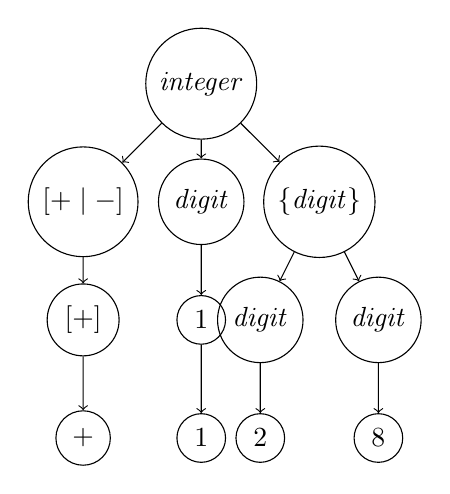
\begin{tikzpicture}[nodes={draw, circle}, ->]

	\node{\textit{integer}}
		child { node {$[+\mid-]$} 
			child { node {[+]}
				child { node {+}}
			}
		}
		child { node {\textit{digit}} 
			child { node {1}
				child { node {1}}
			}
		}
		child { node {\{\textit{digit}\}}
			child { node {\textit{digit}}
				child { node {2}}
			}
			child { node {\textit{digit}}
				child { node {8} }
			}
		};

\end{tikzpicture}
\subsection{Rekursion}
\textit{sequence} $\Leftarrow$ B $\mid$ A\textit{sequence} ergibt "B", "AB", "AAB", $\hdots$\\\\
\textbf{Jede Wiederholung ist eine Rekursion} / kann als Rekursion ausgedrückt werden.\\
\textbf{Nicht jede Rekursion ist eine Wiederholung} / kann man nicht zwingend als Wiederholung ausdrücken.
\subsection{Äquivalenz/Gleichwertigkeit}
Zwei EBNF Beschreibungen sind äquivalent falls sie dieselben legalen und illegalen Symbole erkennen.\\
\begin{tabularx}{\linewidth}{l X}
$\iff$ & Jedes mögliche Symbol, dass eine Regel beschreibt, wird von der anderen als legal bezeichnet, und jedes Symbol dass als illegal erkannt wird wird auch von der anderen als solches erkannt.\\
& Und vice versa. %TODO
\end{tabularx}
\subsection{Sonderzeichen}
Die folgenden 8 Zeichen haben besondere Bedeutungen in EBNF Beschreibungen:\\
\hspace*{1cm} \{, \}, [, ], $\mid$, (, ), $\Leftarrow$\\
Um diese Zeichen in einer Beschreibung zu benutzen, umrahmt man sie.\\
\hspace*{1cm} \fbox{\{}, \fbox{$\mid$}, $\hdots$\\
Man kann auch das Zeichen mit "" umschreiben. In diesem Fall ist auch " ein Sonderzeichen.\\ %TODO
\hspace*{1cm} "\{", "$\mid$", $\hdots$
\newpage
\section{Packages}
package packageName;\\
import packageName.*;\\\\
Klasse mit Namen D in Package a.b.c sollte in a/b/c/D.class gespeichert sein (relativ zu Root von Projekt)
\subsection{Beispiele}
\begin{lstlisting}[language=Java]
	package pacman.model;
	public class Ghost extends Sprite { }

	//Files Ghost.java und Sprite.java
	//sollten im Folder pacman/model sein


	package pacman.gui;
	import pacman.model.*;

	public class PacManGui {
		Ghost blinky = new Ghost();
	}
\end{lstlisting}
\newpage
\section{Access Modifiers}
\begin{tabularx}{\linewidth}{ l X }
\textbf{public} & Sichtbar für alle anderen Klassen.\\
\textbf{private} & Sichtbar nur in dieser Klasse (und ggf. in eingeschlossenen Klassen/Typen).\\
\textbf{protected} & Sichtbar nur in dieser Klasse, allen Unterklassen der Klasse, und allen anderen Klassen/Typen die in dieser Package deklariert sind.\\
\textbf{default} (package) & Sichtbar in dieser Klasse und allen anderen Klassen/Typen die in dieser Package deklariert sind.
\end{tabularx}
\section{Hoare Tripel}
\subsection{Basics} %TODO translate this
\subsection{If-Statements}
\subsubsection{Allgemeine Form}
$\{P\}$ if $\{b\}$ $S1$ else $S2$ $\{Q\}$
\subsubsection{Gültigkeit}
Gültig genau dann, wenn es $\{Q1, Q2\}$ gibt, so dass folgendes gilt:\\\\
\begin{tabular}{ll}
$\{P \land b\}$ $S1$ $\{Q1\}$\\
$\{P \land \neg b \}$ $S2$ $\{Q2\}$\\
$Q1 \lor Q2 \implies Q$
\end{tabular}

\subsection{While-Loops}
\subsubsection{Allgemeine Form}
$\{P\} \text{while}(B) S; {Q}$
\subsubsection{Gültigkeit}
Gültig genau dann, wenn es eine \textbf{Invariante I} gibt, so dass:\\\\
\begin{tabularx}{\linewidth}{lX}
$P \implies I$ & Invariante gilt zu beginn.\\
$\{I \land B\} S \{I\}$ & Nach ausführen des Rumpfes gilt die Invariante wieder.\\
$\{I \land \neg B\} \implies Q$ & Invariante (und Verlassen der Schleife, d.h. test B ist false) impliziert postcondition $Q$.
\end{tabularx}
\newpage
\section{Eclipse}
\subsection{Debugging}
TBD %TODO
\end{document}